\chapter{于iris数据集分类应用研究}
\section{模糊最大熵模型的求解算法}
在描述我们的算法之前,我们首先来定义一些模型的假设:
\[
    \text{n个样本的m维数据集}U:U=\{u_1,u_2,\dots ,u_n\} ,u_i=\{x_1,x_2,\dots,x_m\} \forall i \\
\]
\[
    \text{聚类数}c:2\leqslant c \leqslant n
\]
\[
    \text{隶属度矩阵}A:n\times m\text{的矩阵}
\]
\[
    \text{聚类中心}V:c\times m\text{的矩阵}
\]
模糊最大熵模型的聚类算法步骤如下:\\
输入:原始数据$U$和聚类数$c$\\
输出:隶属度矩阵$A$和聚类中心$V$
\begin{itemize}
    \item[\bf{1)}]首先随机初始化隶属度矩阵并归一化;
    \item[\bf{2)}]根据式\ref{Mvij}计算聚类中心;
    \item[\bf{3)}]计算每一个元素到聚类中心的距离;
    \item[\bf{4)}]根据式\ref{Maij}更新隶属度矩阵;
    \item[\bf{5)}]如果到达指定精度或迭代次数,结束计算过程,否则重复$2\sim 4$步;
    \item[\bf{6)}]输出隶属度矩阵$A$和聚类中心$V$。
\end{itemize}

\section{模型求解}
\par
本文使用的数据是来自UCI的鸢尾花(iris)数据集,这是一个经典的分类数据集,由Iris Setosa(山鸢尾)、Iris Versicolour(杂色鸢尾),以及Iris Virginica(维吉尼亚鸢尾)三种不同类别的鸢尾花组成,
每个样本由四个属性组成,分别是Petal.Length(花瓣长度)、Petal.Width(花瓣宽度)、Sepal.Length(花萼长度)和Sepal.Width(花萼宽度)。
\par 按4.1的算法对iris数据集进行聚类,结果如下:
\begin{table}[!ht]
    \label{聚类中心}
    \caption{聚类中心}
    \centering
    \begin{tabular}{c c c c c}
        \whline & sepal length & sepal width & petal length & petal width \\\whline
        $v_1$   & 5.0136       & 3.3903      & 1.5369       & 0.2781      \\
        $v_2$   & 6.4737       & 2.9437      & 5.1910       & 1.8012      \\
        $v_3$   & 6.0922       & 2.8186      & 4.6775       & 1.5731      \\
        \whline
    \end{tabular}
\end{table}
\begin{figure}[!ht]
    \centering
    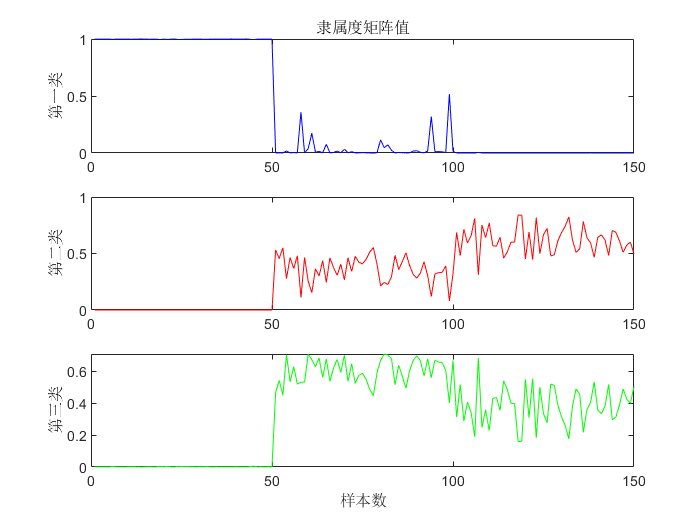
\includegraphics[scale=0.6]{lishudu.png}
    \caption{隶属度矩阵的值}
    \label{隶属度}
\end{figure}
\newpage
\section{与FCM算法分类结果比较}
\begin{table}[!ht]
    \label{准确率比较}
    \caption{准确率比较}
    \centering
    \begin{tabular}{c | c c c c}
        \whline 算法/各类准确率 & Setosa(山鸢尾) & Versicolour(杂色鸢尾) & Virginica(维吉尼亚鸢尾) & 总样本 \\\whline
        FCM                     & 100\%          & 76\%                  & 94\%                    & 90\%   \\
        MFE                     & 100\%          & 86\%                  & 98\%                    & 94.7\% \\
        \whline
    \end{tabular}
\end{table}
从数据的比较中,可以看到模糊最大熵模型相对于FCM算法对iris的数据集分类结果有着更好的表现。